\documentclass[a4j,10pt,uplatex]{jsarticle}

\usepackage[top=30mm, hmargin=20mm, bottom=25mm]{geometry}
\usepackage{ipsj}
\usepackage[dvipdfmx]{graphicx}
% \usepackage[dvipdfmx]{color}
% \usepackage{float}
%\usepackage{wrapfig}
\usepackage{amsmath, amssymb}
\usepackage{amsfonts}
% \usepackage{algorithm}
% \usepackage{algorithmic}
% \usepackage{theorem}
%\usepackage{ulem}
% \usepackage{bld}
%\usepackage{comment}
\usepackage{bm}
% \usepackage[table,xcdraw]{xcolor}
\usepackage[hang,flushmargin]{footmisc}
\usepackage{siunitx}
\sisetup{%
mode = text
}

\renewcommand{\baselinestretch}{0.85}

\graphicspath{{./fig/}}

\renewcommand\thefootnote{*\arabic{footnote}}

\makeatletter
\def\blfootnotetext{\xdef\@thefnmark{}\@footnotetext}

\renewenvironment{thebibliography}[1]
{\section*{\refname\@mkboth{\refname}{\refname}}%
  \list{\@biblabel{\@arabic\c@enumiv}}%
       {\settowidth\labelwidth{\@biblabel{#1}}%
        \leftmargin\labelwidth
        \advance\leftmargin\labelsep
 %\setlength\itemsep{-0.1zh}%←ここの数値を調整(行間のつまり具合)
 %\setlength\baselineskip{7pt}%←ここの数値を調整(追加)(文字の大きさ)
        \@openbib@code
        \usecounter{enumiv}%
        \let\p@enumiv\@empty
        \renewcommand\theenumiv{\@arabic\c@enumiv}}%
  \sloppy
  \clubpenalty4000
  \@clubpenalty\clubpenalty
  \widowpenalty4000%
  \sfcode`\.\@m}
 {\def\@noitemerr
   {\@latex@warning{Empty `thebibliography' environment}}%
  \endlist}
\makeatother

\parindent = 10pt
\setlength\textfloatsep{5pt}

% \newtheorem{theo}{定理}[section]
% \newtheorem{defi}{定義}[section]
% \newtheorem{lemm}{補題}[section]
% \theoremstyle{break}

\newcommand{\UAV}{{\rm UAV}}
\newcommand{\MA}{{\rm MA}}
\newcommand{\argmax}{\mathop{\rm argmax}\limits}
\jtitle{能動推論に基づく1対1インタラクションモデルの検討}
\jcontact{$1$ 東京工業大学 工学院 システム制御系\quad $2$ (株) ホンダ・リサーチ・インスティチュート・ジャパン}
\jauthor{木村 駿希$^1$, 中臺 一博$^1$, 仁科 繫明$^2$, 糸山 克寿$^{1, 2}$}

%本文
\begin{document}

\maketitle

% \blfootnotetext{An Ensemble Method for Multiple Speech Enhancement Using Deep Learning}
% \blfootnotetext{Ryohei Ishii$^1$, Katsutoshi Itoyama$^1$, Kazuhiro Nakadai$^{1, 2}$}
% \blfootnotetext{$1$ Dept.~of Systems and Control Engineering, School of Engineering, Tokyo Institute of % Technology\\
% $2$ Honda Research Institute Japan Co., Ltd.}

\section{はじめに}
人間とコンピュータが対話を行うシステムが近年研究されており,チャットボットを始めとした対話ロボットの需要が高まっている.
例えば坪倉らの研究では,対話ロボットを使用した被験者にアンケートを取ったところ「将来利用したいかどうか」との質問に
対して前向きな回答が多く寄せられている~\cite{坪倉和哉2022}.

対話システムにはタスクの完了を目的としたタスク指向型対話システムと,タスクの完了を目的としない非タスク指向型対話システム(雑談対話システムとも呼ばれる)の2つがあるが,そのどちらも深層学習を用いた手法が盛んである.\cite{東中竜一郎2021}そのため、学習に必要な大量のデータセットが必要である.

さらにテキストによる対話から感情を読み取る研究も盛んに行われているが,驚きや怒りといった感情はテキストに表れにくい上,発話の受け止め方は多種多様なため,テキストでの対話から感情を読み取るのは困難とされている\cite{東中竜一郎2016}.

本研究では大量のデータセットを用いない能動推論を用いた対話モデルを提案する.能動推論とは,推定結果と相手から受け取った信号をもとに行動し,推定結果を更新していく推論方法である.提案モデルでは発話を受け取った際の相手の感情の推定結果と相手からの発話をもとに発話を生成し相手に返すことで,感情推定と対話の成立を同時に行うことができる。
%インタラクションの話(インタラクション関係の論文を集めて問題点を述べる)
%インタラクションのモデル化に取り組んだ
%Q解決する課題を何にするか
%A.報酬がないモデルを作る

\section{能動推論}
自由エネルギー原理とは,Karl J. Fristonが提唱している脳の情報理論である.Fristonは「いかなる自己組織化されたシステムでも,環境内で平衡状態でありつづけるためには,そのシステムの (情報的) 自由エネルギーを最小化しなくてはならない」と定義している.\cite{乾敏郎2019}
自由エネルギー原理では,世界の状態を生物が推測した世界(内部信念)と真の世界(外部環境)との2種類に分けて考える。外部環境から得られた観測信号を用いて目的関数である自由エネルギーを最小化することで,内部信念の分布を外部環境の分布に近づけることが自由エネルギー原理の目的である.この原理は「知覚と行動と学習の統一原理」と言われており,自由エネルギーの最小化によって知覚,行動,学習の最適化を全て行えると考えられており注目されている.

自由エネルギーを応用し,行動選択を説明するための推論を能動推論をいう.能動推論は将来の行動を組み込んだ期待自由エネルギーを最小化するような行動を選択し外部環境に影響を及ぼすことで内部信念を外部環境に近づける推論方法である.ここで推論するのは隠れ状態$(x)$と呼ばれる人間が直接観測することのできない外部環境の要素であり,これは生物が観測できる観測信号$(y)$の原因となるものである.
内部信念の分布$(Q)$,外部環境の分布$(P)$,行動のポリシー(行動計画)$(\pi)$とすると,期待自由エネルギー$(\mathbf{G})$は
\begin{align*}
    \mathbf{G}(\pi) = &\mathbb{E}_{Q(y,x|\pi)}[lnQ(x|\pi) - ln\Tilde{P}(x,y|\pi)] \\
            \ge = &-\mathbb{E}_{Q(y|\pi)}[D_{KL}[Q(x|y,\pi)||Q(x|\pi)]] \\
            &- \mathbb{E}_{Q(y|\pi)}[ln\Tilde{P}(y)]    
\end{align*}
と表現される.なお,$\Tilde{P}$は生物がの望ましいと考えている外部環境の分布である.この式の第一項は観測信号を得る前後の内部信念の差を,第二項はどれだけ望ましい観測信号を得られたかをそれぞれ表す.

能動推論の応用例として2点挙げる.1点目はいわゆるマウンテンカー問題である\cite{mountaincar}.この研究では位置と速度を推定し,目標地点に車が達するように外力を加えている.2点目は環境内の化学物質の濃度を観測し,目標の位置に移動する実験である\cite{mcgregor2015minimal}.エージェントの地点の濃度を観測することで位置を推定し,目標地点まで移動するのを目標としている.

しかし,能動推論を用いたインタラクションモデルを実装した例はあまり多くない.そこで本研究ではchatGTPを利用して能動推論を用いた1対1のインタラクションモデルを実装し,その有効性について検討した.

\section{提案手法}
本研究では1対1のインタラクションモデルとして,親子間の会話モデルを実装した.状況設定として,親は子供に部屋の掃除をさせるための声掛けをし,子供が掃除をすることが目標である.
一方,子供はなるべく部屋の掃除をしたくないが親に叱られることを最も嫌がるため,叱られそうなタイミングを推測して叱られる直前に掃除をすることが目標である.

対話モデルの流れを説明する.まず,親が親自身の感情と行動を出力しChatGTPに渡す.ChatGPTは親の感情と,感情と行動に基づいた発言テンプレートを受け取り自然な対話になるようにテキストを出力する.
出力された親の発言テキストを別のChatGPTが受け取り,Russellの円環モデルに基づいて感情識別を行いarousal値,valence値を出力する.子供は感情値を観測信号として受け取り,親の感情推定,自分の行動選択を能動推論によって行い自身の感情と行動を出力してまた別のchatGPTに渡す.親の時と同様に2つのchatGPTを用いて発言出力,感情識別を行い親に感情値を渡す.親は能動推論を用いず固定関数で次の行動と感情を導出する.
Fig.~\ref{system}に提案モデルの概要を示す.

\begin{figure}[h]
 \centering
 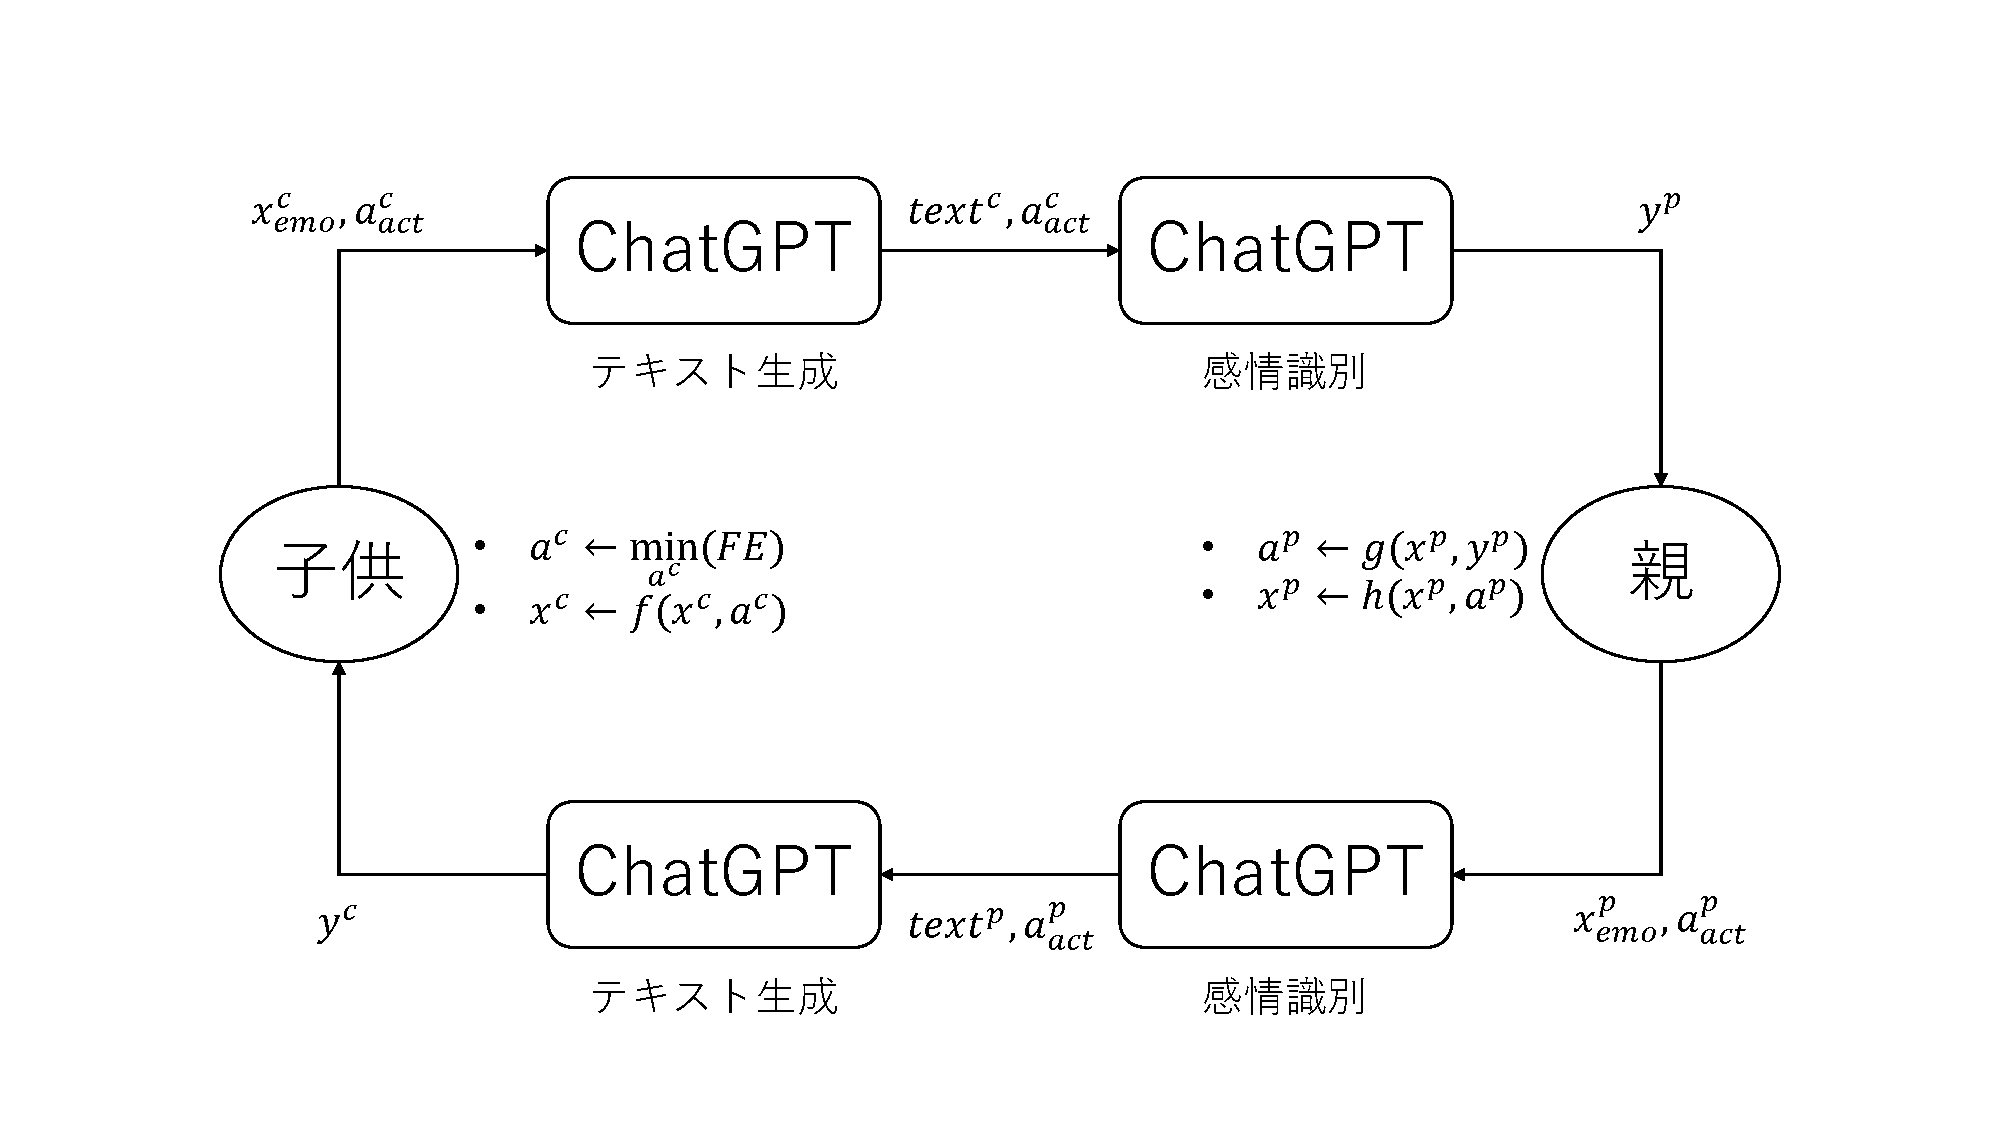
\includegraphics[width=1.\linewidth,pagebox=artbox]{./fig/system.pdf}
 \caption{提案モデルの概要} 
 \label{system}
\end{figure}

この対話モデルでは,能動推論を用いて親の感情を推論することを目的としている.そのため,親の感情を隠れ状態として設定することで,親との対話によって子供が親の感情推定を行うことが望まれる。

\section{実験・考察}
提案手法の有効性を示すために,シュミレーションを行った。
評価指標として,期待自由エネルギー($\mathbf{G}$)の最小値の推移を用いた.
期待自由エネルギー($\mathbf{G}$)は内部信念の分布と外部環境の分布の差を表現するため,
期待自由エネルギーが減少していれば隠れ状態を推測できているといえる.

\begin{figure}[h]
 \centering
 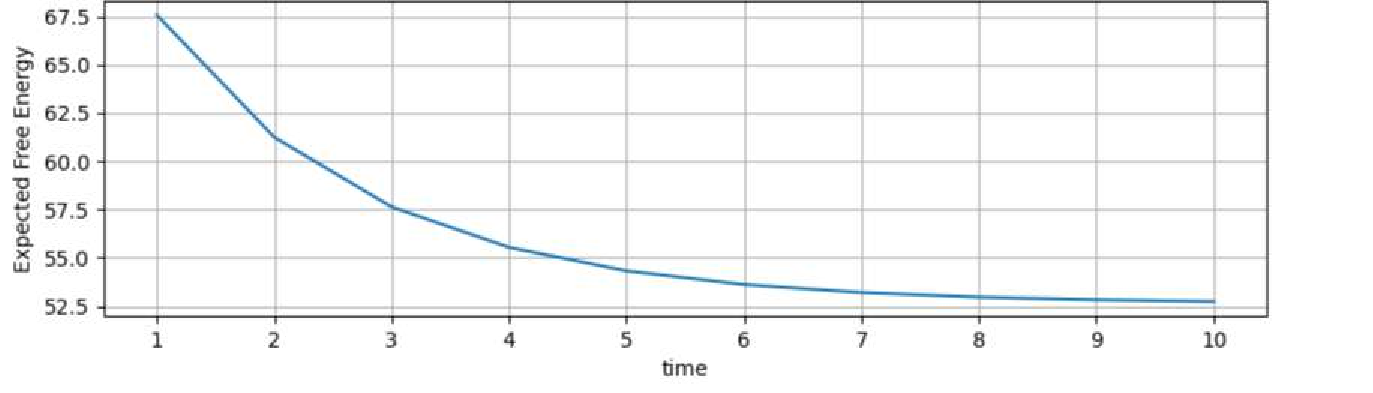
\includegraphics[width=1.\linewidth,pagebox=artbox]{./fig/EFE.pdf}
 \caption{対話モデルにおける期待自由エネルギーの推移} 
 \label{EFE}
\end{figure}

Fig.~\ref{EFE}は対話を10回行った際の期待自由エネルギーの推移である.これより,対話を重ねることで隠れ状態として
設定した親の感情の推定が出来ていることが確認できた。

本手法の特徴として,大量のデータセットを用いて学習することなく対話と推論を同時に行っていることが挙げられる.
隠れ状態と観測信号との尤度分布がわかればどんな状態であっても,自由エネルギーを目的関数として能動推論を行うことで推論と行動選択が
可能とされているため,応用力があると期待されている.

一方,生成モデルの設定が課題の一つとして挙げられる.隠れ状態$x$と観測信号$y$の尤度分布$P(y|x)$と,隠れ状態と行動$a$との遷移分布$P(x_t|x_{t-1}, a_{t-1})$を予め設定する必要があり,隠れ状態,観測信号,行動の関係を知っていなければならない.そのため,関係を把握しきれない複雑な設定に本研究では対応できていない.解決策として,生成モデルの更新をすることが考えられる.行動して得られる感覚信号に応じて生成モデルを更新することが出来れば未知の関係がある設定に対しても能動推論が行えると期待している.



\section{おわりに}
本研究では,能動推論を用いた1対1のインタラクションモデルを提案した.モデルを実装し,シュミレーション実験を
行うことで対話モデルの有効性を示した.

% \paragraph{謝辞}
% 本研究はJSPS科研費 JP19K12017, JP19KK0260 および JP20H00475 の助成を受けた.

\footnotesize
\bibliographystyle{junsrt}   
\bibliography{cite}    % bibファイル名を指定する.拡張子は除く.

\end{document}
